% !TEX program = pdflatex
% !TEX options = -synctex=1 -interaction=nonstopmode -file-line-error "%DOC%"
% 作业模板
\documentclass[UTF8,10pt,a4paper]{article}
\usepackage{ctex}
\newfontfamily\menlo{MONACO.TTF}
\usepackage{amsmath}
\usepackage{diagbox}
\usepackage{float}
\usepackage{listings}
\usepackage{multirow}
\usepackage{tabularx}

\usepackage{url}
\usepackage{xcolor}
\newcommand{\tabincell}[2]{\begin{tabular}{@{}#1@{}}#2\end{tabular}}

\lstset{
    breaklines,                                 % 自动将长的代码行换行排版
    extendedchars=false,                        % 解决代码跨页时,章节标题,页眉等汉字不显示的问题
    backgroundcolor=\color[rgb]{0.96,0.96,0.96},% 背景颜色
    keywordstyle=\color{blue}\bfseries,         % 关键字颜色
    identifierstyle=\color{black},              % 普通标识符颜色
    commentstyle=\color[rgb]{0,0.6,0},          % 注释颜色
    stringstyle=\color[rgb]{0.58,0,0.82},       % 字符串颜色
    showstringspaces=false,                     % 不显示字符串内的空格
    numbers=left,                               % 显示行号
    numberstyle=\tiny\menlo,                    % 设置数字字体
    basicstyle=\small\menlo,                    % 设置基本字体
    captionpos=t,                               % title在上方(在bottom即为b)
    frame=single,                               % 设置代码框形式
    rulecolor=\color[rgb]{0.8,0.8,0.8},         % 设置代码框颜色
}  

\usepackage{pythonhighlight}
\usepackage{listings}
\usepackage{xcolor}
\usepackage{graphicx}
\usepackage[a4paper,left=2cm,right=2cm,top=2cm,bottom=2cm]{geometry}
\usepackage{fancyhdr}
% \catcode`\。=\active
% \newcommand{。}{.}
\newcommand{\CourseName}{操作系统(Operating System)}
\newcommand{\CourseCode}{CS307 \& CS356}
\newcommand{\Semester}{2020-2021学年第二学期}
\newcommand{\ProjectName} {\Huge{Project 1}} 
\newcommand{\StudentName}{刘涵之}
\newcommand{\StudentID}{519021910102}
\usepackage[vmargin=1in,hmargin=.5in]{geometry}
\usepackage{fancyhdr}
\usepackage{lastpage}
\usepackage{calc}
\pagestyle{fancy}
\fancyhf{}
\fancyhead[L]{\CourseName}
\fancyhead[C]{\ProjectName}
\fancyhead[R]{\StudentName}
\fancyfoot[R]{\thepage\ / \pageref{LastPage}}
\setlength\headheight{12pt}
\fancypagestyle{FirstPageStyle}{
    \fancyhf{}
    \fancyhead[L]{\CourseName\\
        \CourseCode\\
        \Semester}
    \fancyhead[C]{\large\bfseries\ProjectName \\}
    \fancyhead[R]{Name: \makebox[\widthof{\StudentID}][s]{\StudentName}\\
        ID : \StudentID\\
        }
    \fancyfoot[R]{\thepage\ / \pageref{LastPage}}
    \setlength\headheight{36pt}
}
\usepackage{amsmath,amssymb,amsthm,bm}
\allowdisplaybreaks[4]
\newtheoremstyle{Problem}
{}
{}
{}
{}
{\bfseries}
{.}
{ }
{第\thmnumber{ #2}\thmname{ #1}\thmnote{ (#3)} 得分: \underline{\qquad\qquad}}
\theoremstyle{Problem}
\newtheorem{prob}{题}
\newtheoremstyle{Solution}
{}
{}
{}
{}
{\bfseries}
{:}
{ }
{\thmname{#1}}
\makeatletter
\def\@endtheorem{\qed\endtrivlist\@endpefalse}
\makeatother
\theoremstyle{Solution}
\newtheorem*{sol}{解}
% \usepackage{graphicx}
\title{Project 1: Introduction to Linux Kernel Modules}
\date{}
\begin{document}
\maketitle
\thispagestyle{FirstPageStyle}
\section{Prepare Experiment Environment}
In this section, I use VMware WorkStation to install the Ubuntu operating system. Then, I compile and upgrade the linux kernel to the latest version (5.11.3).
\subsection{VMware WorkStation and Ubuntu OS}
I install the \textbf{VMware Workstation 16 Pro} and download the image of Ubuntu OS (\textbf{ubuntu-20.04.2.0-desktop-amd64.iso}). I create a new virtual machine and choose this image to install.

\begin{figure}[H]
\begin{minipage}[H]{0.5\linewidth}
    \centering
    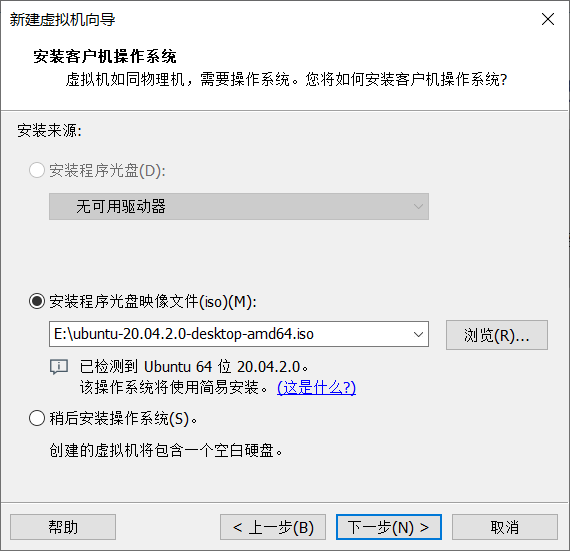
\includegraphics[width=160pt]{1.png}
    \caption{VMware WorkStation}
    \label{1}
\end{minipage}
\begin{minipage}[H]{0.5\linewidth}
    \centering
    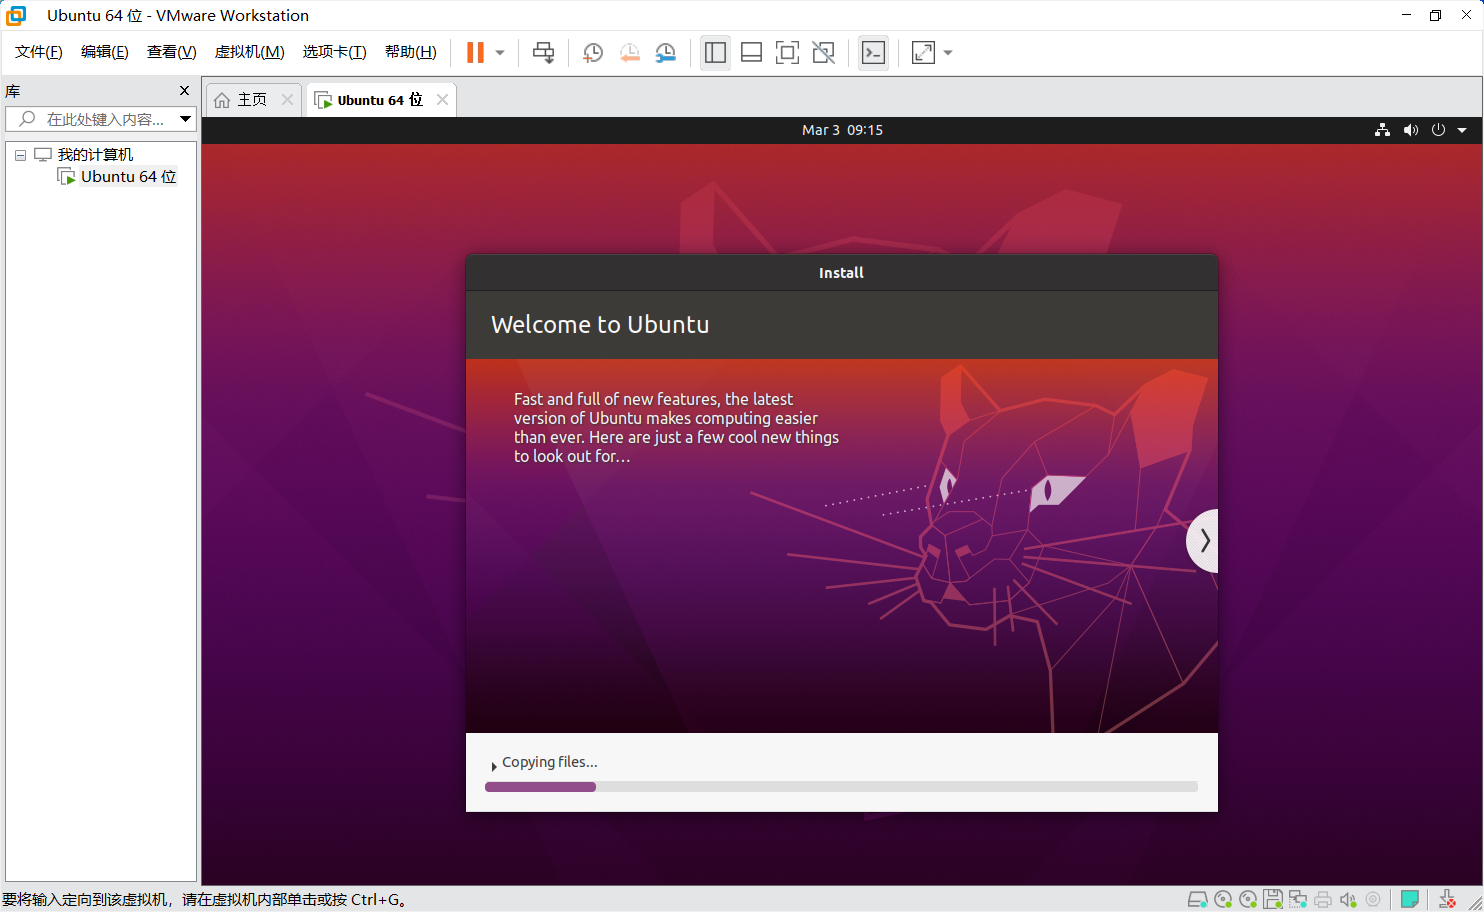
\includegraphics[width=230pt]{2.png}
    \caption{Install Ubuntu OS}
    \label{2}
\end{minipage}
\end{figure}

Then I check the version of linux kernel, using the following instruction in bash.

\begin{lstlisting}
uname -a
\end{lstlisting}

\begin{figure}[H]
    \centering
    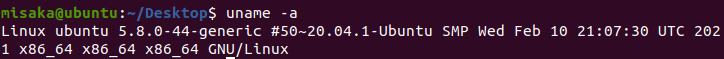
\includegraphics[width=380pt]{3.png}
    \caption{Check the Kernel Version}
    \label{3}
\end{figure}

In Figure \ref{3}, it shows that the current kernel version is \textbf{5.8.0}.

\subsection{Change the Package Source}
To download packages more faster, i change the source of the system package manager to SJTUG source. I follow the document in \underline{https://mirror.sjtu.edu.cn/docs/ubuntu} and using the following instructions.

\begin{lstlisting}
sudo gedit /etc/apt/sources.list
\end{lstlisting}

\begin{lstlisting}
deb https://mirrors.sjtug.sjtu.edu.cn/ubuntu focal main restricted
deb https://mirrors.sjtug.sjtu.edu.cn/ubuntu focal-updates main restricted
deb https://mirrors.sjtug.sjtu.edu.cn/ubuntu focal universe
deb https://mirrors.sjtug.sjtu.edu.cn/ubuntu focal-updates universe
deb https://mirrors.sjtug.sjtu.edu.cn/ubuntu focal multiverse
deb https://mirrors.sjtug.sjtu.edu.cn/ubuntu focal-updates multiverse
deb https://mirrors.sjtug.sjtu.edu.cn/ubuntu focal-backports main restricted universe multiverse
deb http://archive.canonical.com/ubuntu focal partner
deb https://mirrors.sjtug.sjtu.edu.cn/ubuntu focal-security main restricted universe multiverse
\end{lstlisting}

\begin{lstlisting}
sudo apt update
sudo apt upgrade
\end{lstlisting}

To prepare for compiling, i need to install some packages essential for building.

\begin{lstlisting}
sudo apt-get install kernel-package git fakeroot build-essential
sudo apt-get install ncurses-dev xz-utils libssl-dev bc flex bison
\end{lstlisting}


\subsection{Compile and Upgrade Linux Kernel (Recommended)}
To understand how kernel is installed, I decide to upgrade my kernel.

I find the latest release of linux kernel on \underline{www.kernel.org}

\begin{figure}[H]
    \centering
    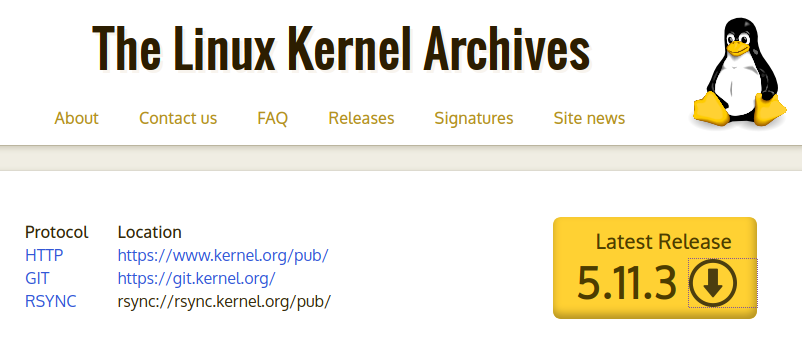
\includegraphics[width=300pt]{4.png}
    \caption{the Latest Kernel Version}
    \label{4}
\end{figure}

I download the \textbf{linux-5.11.3.tar.xz} and then move it to \textbf{/usr/src}

\begin{lstlisting}
cp linux-5.11.3.tar.xz /usr/src
\end{lstlisting}

Then i unzip the file using the following instructions.

\begin{lstlisting}
sudo xz -d linux-5.11.3.tar.xz
sudo tar xvf linux-5.11.3.tar
\end{lstlisting}

\begin{figure}[H]
    \centering
    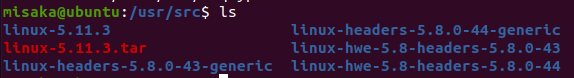
\includegraphics[width=380pt]{5.png}
    \caption{File in /usr/src}
    \label{5}
\end{figure}

Then i use the following instruction to set the configurations, the menu is displayed as Figure \ref{6}. I use the default configurations.

\begin{lstlisting}
sudo make menuconfig
\end{lstlisting}

\begin{figure}[H]
    \centering
    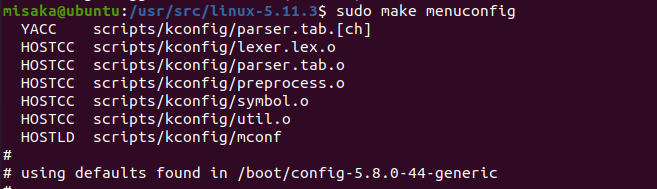
\includegraphics[width=380pt]{7.png}
    \caption{sudo make menuconfig}
    \label{7}
\end{figure}

\begin{figure}[H]
    \centering
    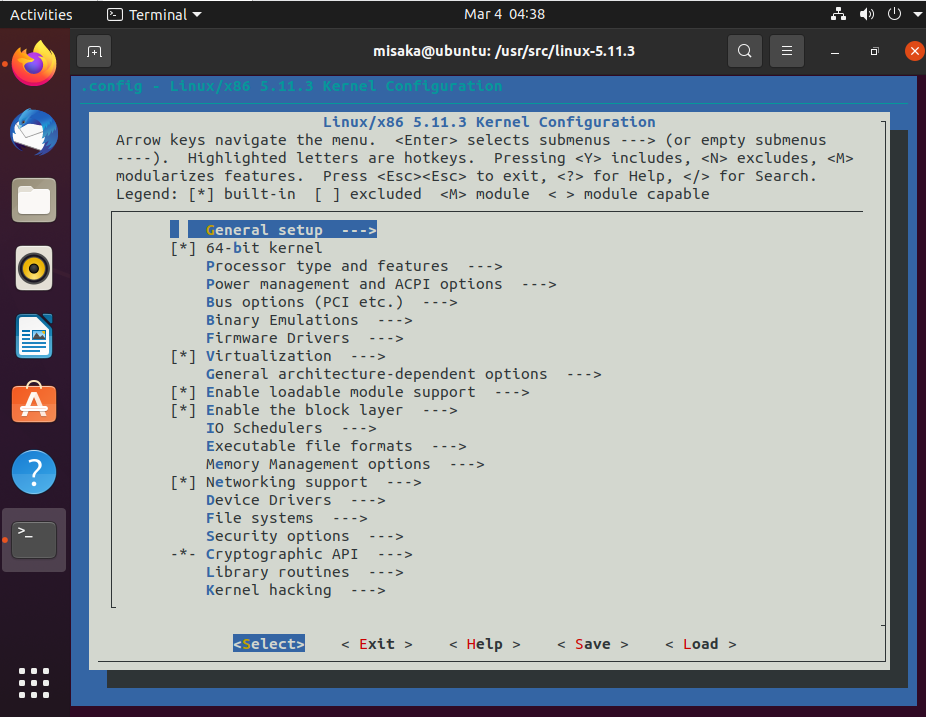
\includegraphics[width=380pt]{6.png}
    \caption{Menu of configurations}
    \label{6}
\end{figure}

Finally, i run the following instruction to compile the kernel with 8 threads compile in parallel.

\begin{lstlisting}
sudo make -j8
\end{lstlisting}

After 30 minutes, the compilation is complete.

\begin{figure}[H]
    \centering
    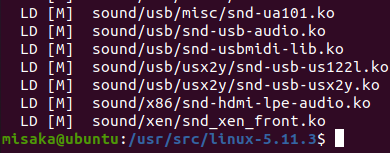
\includegraphics[width=280pt]{9.png}
    \caption{sudo make -j8}
    \label{9}
\end{figure}

I run the following instruction to install modules.

\begin{lstlisting}
sudo make modules_install
\end{lstlisting}

\begin{figure}[H]
    \centering
    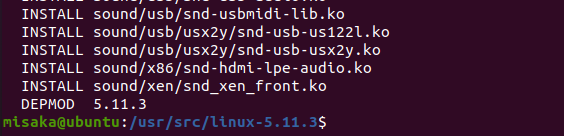
\includegraphics[width=280pt]{10.png}
    \caption{sudo make modules\_install}
    \label{10}
\end{figure}

Then i can install the new kernel!

\begin{lstlisting}
sudo make install
\end{lstlisting}

\begin{figure}[H]
    \centering
    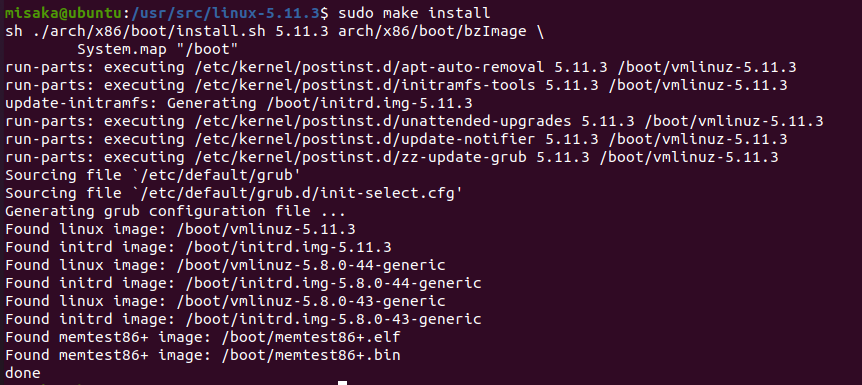
\includegraphics[width=400pt]{11.png}
    \caption{Install the new kernel}
    \label{11}
\end{figure}

Then i reboot the system and check the kernel version again. It shows that the new kernel (5.11.3) is installed successfully.

\begin{figure}[H]
    \centering
    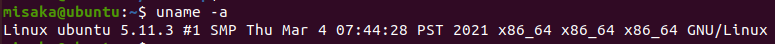
\includegraphics[width=420pt]{12.png}
    \caption{Check the new kernel}
    \label{12}
\end{figure}

% \begin{prob}[问题标题]
%     此乃问题描述。
% \end{prob}
% \begin{sol}
%     此为解。
% \end{sol}

\section{Kernel Modules Overview}
In this section i will talk about the programming project at the end of Chapter 2.
\subsection{Task 1 - Simple Module}

I use the following commands to make and install my module (for Task 2 & 3, all most the same).
\begin{lstlisting}
sudo make
sudo dmesg -C
sudo insmod simple.ko
dmesg
sudo rmmod simple
dmesg
\end{lstlisting}


In the Simple module, we are required to print the \textbf{Golden Ratio Prime} when initializing (simple\_init()) and print the \textbf{greatest common divisor} of 3300 and 24 when exiting (simple\_exit()).

As written on the textbook, i find the constant GOLDEN\_RATIO\_PRIME in the <linux/hash.h> and gcd() in the <linux/hash.h>. The code of simple.c is displayed as follows.

\begin{lstlisting}[language = c]
#include <linux/init.h>
#include <linux/module.h>
#include <linux/kernel.h>
#include <linux/hash.h>
#include <linux/gcd.h>

int simple_init(void)
{
       printk(KERN_INFO "Loading Module\n");
       printk(KERN_INFO "GOLDEN_RATIO_PRIME: %llu\n", GOLDEN_RATIO_PRIME);
       return 0;
}

void simple_exit(void) {
	printk(KERN_INFO "GCD(3300, 24) = %lu\n", gcd(3300,24));
	printk(KERN_INFO "Removing Module\n");
}

module_init( simple_init );
module_exit( simple_exit );

MODULE_LICENSE("GPL");
MODULE_DESCRIPTION("Simple Module");
MODULE_AUTHOR("MisakaCenter");
\end{lstlisting}

For this task, the \textbf{Makefile} is written as follows.
\begin{lstlisting}
obj-m := simple.o
all:
	make -C /usr/src/linux-5.11.3/ M=$(shell pwd) modules
clean:
	make -C /usr/src/linux-5.11.3/ M=$(shell pwd) clean
\end{lstlisting}


The result is shown as follows.
\begin{figure}[H]
    \centering
    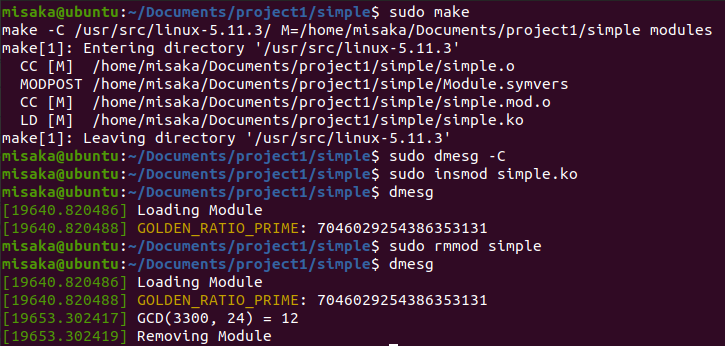
\includegraphics[width=380pt]{simple1.png}
    \caption{simple.ko}
    \label{88}
\end{figure}


More over, for preparation of the Task 2, i add the following code to the simple\_init.
\begin{lstlisting}[language = c]
printk(KERN_INFO "(Loading) Jiffies: %lu\n", jiffies);
printk(KERN_INFO "HZ: %d\n", HZ);
\end{lstlisting}

and i add the following code to the simple\_exit.
\begin{lstlisting}[language = c]
printk(KERN_INFO "(Removing) Jiffies: %lu\n", jiffies);
\end{lstlisting}

The result is shown as follows.
\begin{figure}[H]
    \centering
    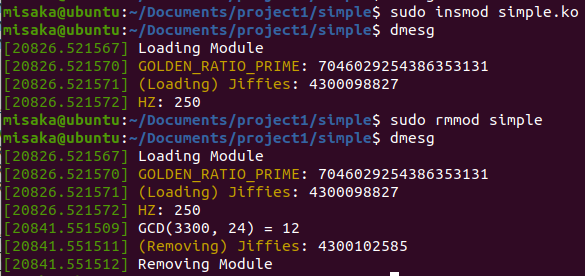
\includegraphics[width=380pt]{simple2.png}
    \caption{Print jiffies and HZ}
    \label{7}
\end{figure}

\subsection{Task 2 - Jiffies Module}

Design a kernel module that creates a /proc file named /proc/jiffies that reports the current value of jiffies when the /proc/jiffies file is read.

As same as Task 1, jiffies can be get in <linux/jiffies.h>, and its type is unsigned long volatile. We can use \%lu to format its output. The code of jiffies.c is display as follows.
\begin{lstlisting}[language = c]
#include <linux/init.h>
#include <linux/module.h>
#include <linux/kernel.h>
#include <linux/proc_fs.h>
#include <asm/uaccess.h>
#include <linux/jiffies.h>

#define BUFFER_SIZE 128

#define PROC_NAME "jiffies"

ssize_t proc_read(struct file *file, char *buf, size_t count, loff_t *pos);

static struct proc_ops proc_ops = {
        .proc_read = proc_read
};

int proc_init(void)
{
        proc_create(PROC_NAME, 0, NULL, &proc_ops);
        printk(KERN_INFO "/proc/%s created\n", PROC_NAME);
	return 0;
}

void proc_exit(void) {
        remove_proc_entry(PROC_NAME, NULL);
        printk( KERN_INFO "/proc/%s removed\n", PROC_NAME);
}

ssize_t proc_read(struct file *file, char __user *usr_buf, size_t count, loff_t *pos)
{
        int rv = 0;
        char buffer[BUFFER_SIZE];
        static int completed = 0;
        if (completed) {
                completed = 0;
                return 0;
        }
        completed = 1;
        rv = sprintf(buffer, "jiffies: %lu\n", jiffies);
        copy_to_user(usr_buf, buffer, rv);
        return rv;
}

module_init( proc_init );
module_exit( proc_exit );

MODULE_LICENSE("GPL");
MODULE_DESCRIPTION("Jiffies Module");
MODULE_AUTHOR("MisakaCenter");
\end{lstlisting}


For this task, the \textbf{Makefile} is written as follows.
\begin{lstlisting}
obj-m := jiffies.o
all:
	make -C /usr/src/linux-5.11.3/ M=$(shell pwd) modules
clean:
	make -C /usr/src/linux-5.11.3/ M=$(shell pwd) clean
\end{lstlisting}

The result is shown as follows.
\begin{figure}[H]
    \centering
    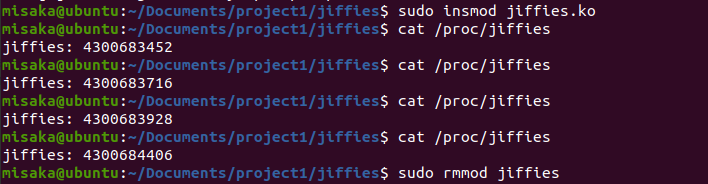
\includegraphics[width=380pt]{jiff.png}
    \caption{Jiffies Module}
    \label{7223}
\end{figure}

\subsection{Task 3 - Seconds Module}
Design a kernel module that creates a proc file named /proc/seconds that reports the number of elapsed seconds since the kernel module was loaded. This will involve using the value of jiffies as well as the HZ rate.

To solve this task:
\begin{itemize}
    \item When initializing, record the current jiffies in the global variable \textbf{jiffies\_load}
    \item jiffies / HZ turns out to be seconds
    \item when /proc/seconds is read, (jiffies−jiffies\_load)/HZ is the seconds we need.
\end{itemize}

The code of seconds.c is display as follows.
\begin{lstlisting}[language = c]
#include <linux/init.h>
#include <linux/module.h>
#include <linux/kernel.h>
#include <linux/proc_fs.h>
#include <asm/uaccess.h>
#include <linux/jiffies.h>
#include <asm/param.h>

#define BUFFER_SIZE 128

#define PROC_NAME "seconds"

unsigned long jiffies_load;

ssize_t proc_read(struct file *file, char *buf, size_t count, loff_t *pos);

static struct proc_ops proc_ops = {
        .proc_read = proc_read
};

int proc_init(void)
{
        proc_create(PROC_NAME, 0, NULL, &proc_ops);
        printk(KERN_INFO "/proc/%s created\n", PROC_NAME);
        jiffies_load = jiffies;
	return 0;
}

void proc_exit(void) {
        remove_proc_entry(PROC_NAME, NULL);
        printk( KERN_INFO "/proc/%s removed\n", PROC_NAME);
}

ssize_t proc_read(struct file *file, char __user *usr_buf, size_t count, loff_t *pos)
{
        int rv = 0;
        char buffer[BUFFER_SIZE];
        static int completed = 0;
        unsigned long seconds_since_load = (jiffies - jiffies_load )/ HZ;
        if (completed) {
                completed = 0;
                return 0;
        }
        completed = 1;
        rv = sprintf(buffer, "The number of seconds: %lu\n", seconds_since_load);
        copy_to_user(usr_buf, buffer, rv);
        return rv;
}

module_init( proc_init );
module_exit( proc_exit );

MODULE_LICENSE("GPL");
MODULE_DESCRIPTION("Seconds Module");
MODULE_AUTHOR("MisakaCenter");
\end{lstlisting}


For this task, the \textbf{Makefile} is written as follows.
\begin{lstlisting}
obj-m := seconds.o
all:
	make -C /usr/src/linux-5.11.3/ M=$(shell pwd) modules
clean:
	make -C /usr/src/linux-5.11.3/ M=$(shell pwd) clean
\end{lstlisting}


The result is shown as follows.
\begin{figure}[H]
    \centering
    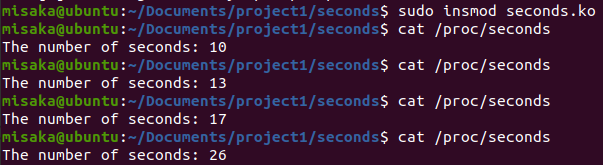
\includegraphics[width=380pt]{sec.png}
    \caption{Seconds Module}
    \label{722ds3}
\end{figure}
\end{document}